\subsection{CI/CD}
\label{cicd:label}

{\color{red} \textbf{XXXXoOChangeThis}}

This section will clarify choices and reflections in the pipeline .yml file, which is found in Appendix[XXXXoOChangeThis]. The technology choice for our pipeline was Travis CI. The technology is easily integratable with Github, making it easy to get it up and running. Before the pipeline executes each stage, it sets up the environment: Stating that it is a Csharp project, a version of dot net. Followed by setting up sonar cloud for maintenance checking, which branches to build on, setting up SSH, installing docker \& node and finally declaring the stages the pipeline should complete concluding a successful build.

\subsubsection*{Pipeline stages}

\begin{enumerate}
  \item[1.] build\_and\_unittest\_analysis: Builds the project, ensures no static analysis errors. Runs all the unit tests in the system. If successful, runs sonar cloud scan for vulnerabilities and evaluates the code quality etc, which the team can inspect.
  \item[2.] docker\_build: Builds the docker image and pushes it to DockerHub.
  \item[3.] docker\_scan\_containers: SSH's into the Digital Ocean server pulls+scans the previously created docker image. If any critical vulnerability is found in the script will fail the build.
  \item[4.] deploy: This stage only happens if code is pushed to the team's "release branch" this acts as continuous delivery. We only manually integrate push to the release branch after reviewing the builds completed in the main branch. The stage ssh's into the server, pulls the most recent images and redeploys the docker containers.
\end{enumerate}

\subsubsection*{Pipeline reflections}

If we were to further develop on the systems pipeline, the team would add a "staging environment" to further test the system before releasing to production as seen in figure[INSERT FIGURE REFERENCE]:


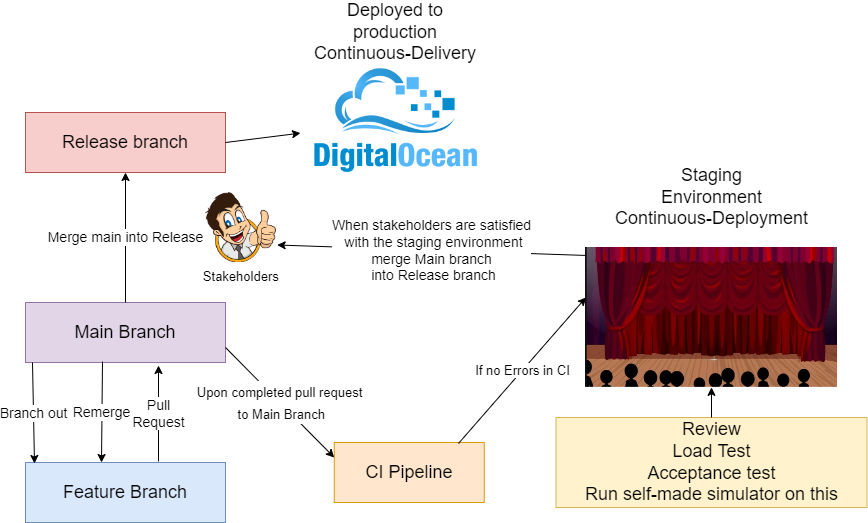
\includegraphics[width=8cm, height=6cm]{images/image.PNG}

The branching strategy as previously in discussed section[INSERT SECTION] remains intact. Upon completion of a newly implemented feature and a approved build state from the CI pipeline, the infrastructure "Continiously Deploys" the new version of the system into a staging environment. In this environment the team will run acceptence tests, review the code and run load tests in order to see if we are compliant with the requirements of the simulator. When sufficient testing has been done of the system, the team will merge the main branch into the release branch triggering the "Continious Delivery", which will deploy the delivery to production. As a potential last edition to the pipeline, the team has considered building its own simulator which would run against the staging environment in order to simulate the real world, this would further enhance the chances of no errors occouring once deployed to production. In general, creating the staging environment will result in the users of the frontend experiencing less errors as the system is tested more thoroughly and the simulator would detect no errors, granted that our tests in the staging environment are sufficient.\\ 

We conclude that the pipeline has been successful. It is the backbone of the DevOps infrastructure in our system. However, the team did experience some troubles with Travis CI, which would make the team consider other technologies in future projects. Travis CI used more credits than first anticipated which is a problem as the team is on low funding. In addition to the credits, connecting to remote servers was troublesome in Travis. All of the functionality works with Travis, but if we were to implement it again the team would have chosen Jenkins or Github actions, which are two very popular CI/CD tools. Jenkins seemed of most interest as it is decoupled from our Version Control server, and we are able to host it ourselves, which means we are not vendor-bound in any way.\\

If our DevOps skills were to improve further, creating the staging environment could become redundant: the systems CI pipeline could potentially fully automate spinning up a temporary staging-environment-server and running load tests and acceptance tests automatically.